\chapter{Contexte Entreprise}
\section{Entreprise d'accueil}
L’accueil téléphonique en France est principalement utilisé par les professions libérales 
mais également pour les entreprises de toutes tailles souhaitant avoir un accueil téléphonique.
Cette profession dispose de sa chambre professionnelle  le « SIST » qui regroupe 60 centres d’accueil partout en France cela représente 
8000 hôtesses d'accueil téléphonique et 150 millions d'appels entrant traités par an. 
Le principe de l’accueil téléphonique est de ne rater aucun appel téléphonique 
pour ne pas perdre de potentiel client. \newline

Le fait de confier sa ligne téléphonique à des professionnels 
permet d’avoir un accueil téléphonique de qualité et permet également de réduire drastiquement les coûts qu’aurait une entreprise à engager 
une ou plusieurs personnes à temps plein pour répondre aux appels.\newline

Créée en 1992 par ses actuels dirigeants, Eurice est spécialisée dans la gestion d'appels entrants 
et est à la fois opérateur et fournisseur de solutions techniques de par ses services:
\begin{itemize}
	\item L'accueil téléphonique fourni par un plateau de réception des appels 
	au sein des locaux de l'entreprise, qui peut aussi parfois servir d’environnement de pré-production 
	avant le déploiement de mise à jour chez les centres d'appels client.

	\item Le développement de solutions pour les centres d'appels: logiciel de gestion d'agenda, 
	répartiteur d'appel, portail client et applications mobiles, tous les logiciels utilisés à Eurice 
	et vendus au client, cela permet entre autre de connaître le besoin avec plus de précision 
	car nous sommes clients de nos propres produits.
\end{itemize}
Chaque année, Eurice gère pour le compte de ses clients près 
d'un million d'appels décrochés en moins de 3 sonneries.

\begin{figure}[h]
	\centering
	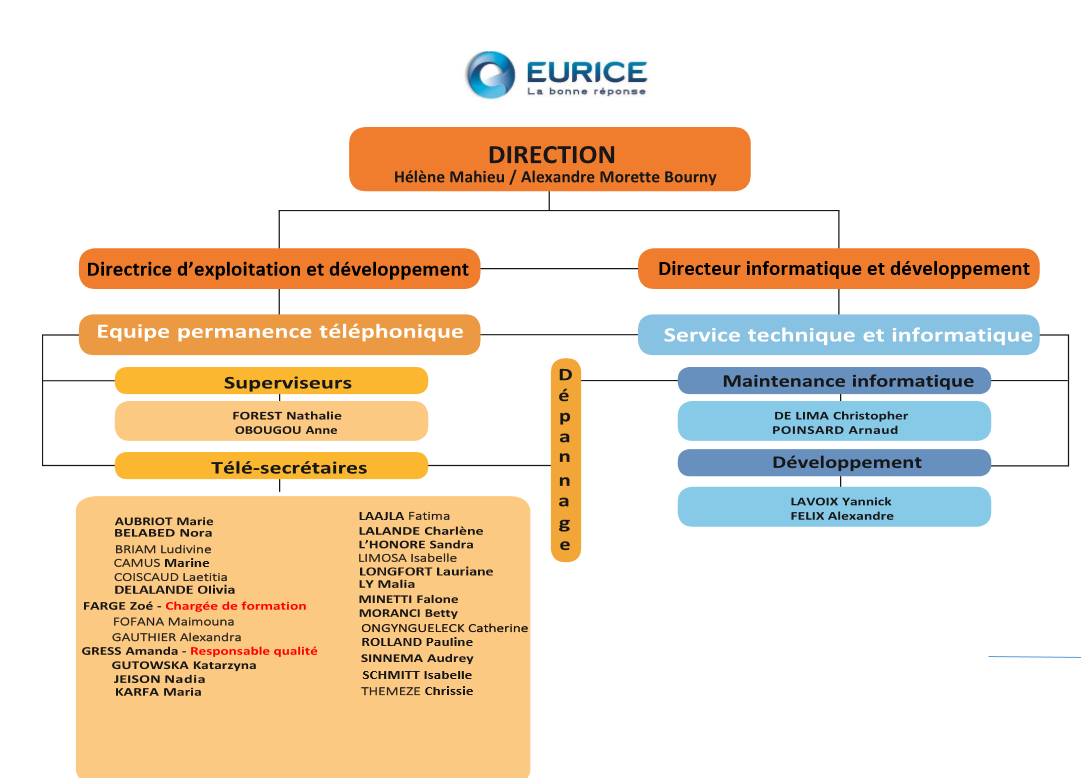
\includegraphics[width=0.7\linewidth]{Images/organigramme_fonctionnel}
	\caption{Organigramme Fonctionnel}
	\label{fig:organigrammefonctionnel}
\end{figure}

\section{Contexte Métier}

\subsection{Callibri}
Il s'agit de l'application principale pour un centre d'appel. 
Ce logiciel permet la gestion de plusieurs dossiers avec leur agenda, 
avoir une communication entre la secrétaire et le client via les instructions et les messages. 
un système de scripting soutient l'opératrice lors du traitement d'un appel, 
c'est le support du pré-traitement et du post-traitement de l'appel. \newline

\gls{Callibri} s'interface avec le système d'appel pour automatiquement ouvrir le dossier correspondant 
au numéro appelé, cela permet de gagner un temps conséquent 
et de rendre transparent l'appel au yeux de l'appelant qui ne sait pas 
que son appel est décroché dans un centre d'appel. \newline


L'application utilise pour la majeure partie de l'interface des pages web grâce 
à la librairie Essentials Objects utilisant un moteur chrome embarqué.
Le reste de l'interface qui comprend le menu et la fenêtre native est réalisé en WPF.
\newline


\gls{Callibri} étant utilisé sur plusieurs postes accédant à des ressources communes, 
le logiciel communique via messages UDP aux autres postes, pour, par exemple, éviter de prendre 
un rendez-vous sur le même créneau libre.

\section{Focus sur le service du stage}
Je fais partie de l'équipe développement qui est composé de Yannick Lavoix et de moi-même, 
notre objectif est d'ajouter des fonctionnalités aux logiciels existant, 
les maintenir et créer de nouvelles solutions. notre interlocuteur principal est le directeur
de l'entreprise Mr. Morette-Bourny, nous sommes parfois mis en relation avec des clients 
ou des partenaires tel que RDVMedicaux ou Doctolib. \newline

\subsection{Callibri Mobile}
Callibri Mobile est l'application android et iOS qui permet aux clients finaux 
d'acceder à leur agenda depuis leur téléphone, il ne s'agit pas d'une version 
responsive du web2 utilisé pas un wrapper pour faire une application mais bien
une application indépendantes et optimisé pour l'expérience smartphone,
il s'agit du projet principal de mes 2 années d'alternance à l'ESGI et ma première 
application mobile en production utilisé par plusieurs centaines de clients.
\newpage

\subsection{Site Client "Web2"}
le site client, portant le dénomination web2, permet l'accès aux 
clients finaux (practiciens dans le médical principalement) à leurs agenda,
il a été développé an ASP.Net 4.5 avec un front-end html + css + js avec jquery.
ce projet peut être considéré comme ayant du code legacy car il n'y a aucun 
test unitaires, aucune documentation et le code ne respecte pas la majorité
des principes basiques de la programmation orienté objet. 
\newline

\begin{figure}[!h]
    \centering
    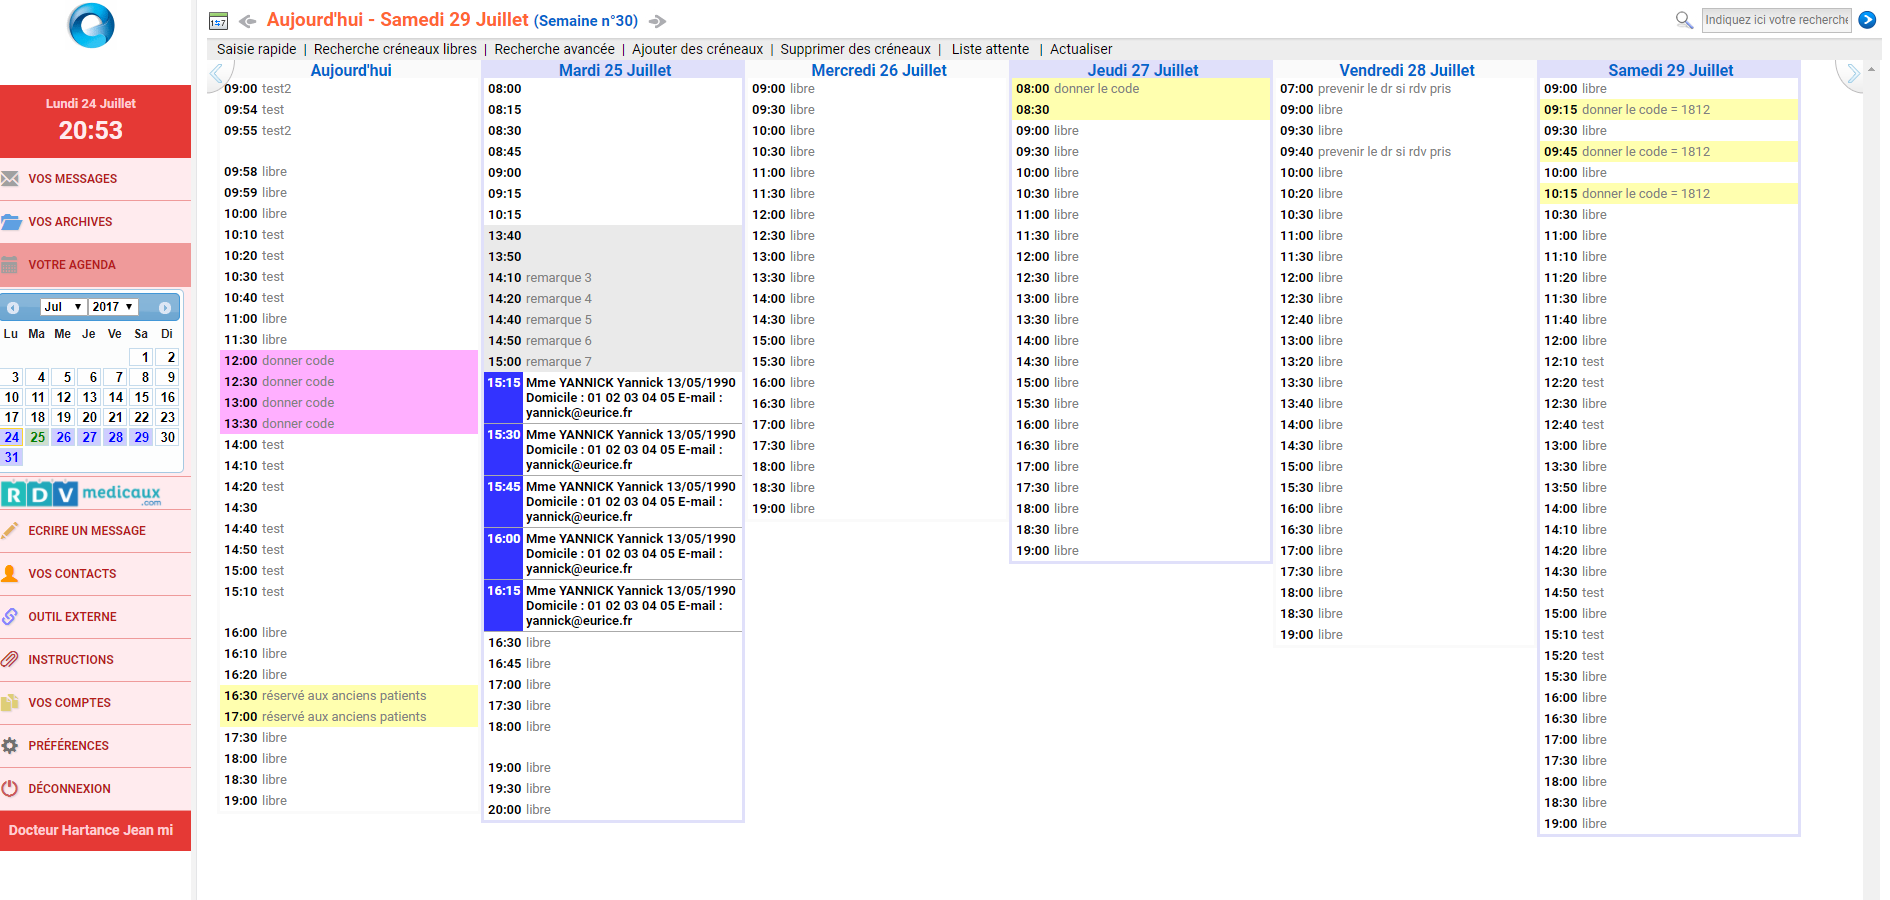
\includegraphics[width=1\linewidth]{Images/web2agenda}
    \caption{Agenda du web2}
    \label{fig:archhexa}
\end{figure}


\begin{figure}[!h]
    \centering
    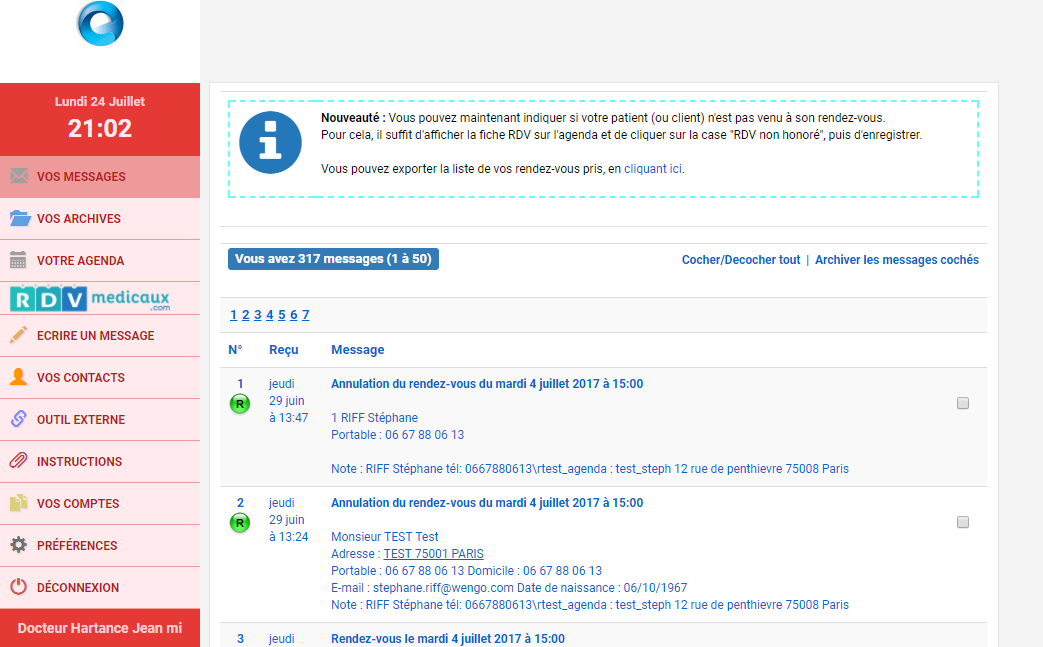
\includegraphics[width=0.8\linewidth]{Images/web2messages}
    \caption{interface des messages du web2}
    \label{fig:archhexa}
\end{figure}

